\documentclass{beamer}
%\usetheme{metropolis}
\usetheme{default}
\usecolortheme{default} % change this to change the color scheme
\usepackage{graphicx}
\usepackage{amsthm}
\setbeamertemplate{itemize items}[circle]
\usepackage{booktabs}
\usepackage{hyperref}
\usepackage{listings}
%\newtheorem{assumption}{Assumption}
\newtheorem{assumption}{Assumption}[section]
\colorlet{shadecolor}{gray!40}
\newtheoremstyle{plain} % Just using 'plain' or any name if you're not defining a style
{}    % Space above
{}    % Space below
{\itshape} % Body font
{}    % Indent amount
{\bfseries} % Theorem head font
{.}   % Punctuation after theorem head
{.5em} % Space after theorem head
{}    % Theorem head spec (completely empty, no predefined format)

\theoremstyle{plain}
\newtheorem*{customthm}{} % No predefined name

% Command to insert theorem with just a title
\newcommand{\customtheorem}[2]{
	\begin{customthm}
		\textbf{#1.} #2
	\end{customthm}
}

\lstset{
	language=R,
	basicstyle=\ttfamily\small,
	commentstyle=\color{black},
	keywordstyle=\color{blue},
	numbers=left,
	numberstyle=\tiny\color{red},
	stepnumber=1,
	numbersep=5pt,
	backgroundcolor=\color{shadecolor},
	showspaces=false,
	showstringspaces=false,
	showtabs=false,
	frame=single,
	tabsize=2,
	captionpos=b,
	breaklines=true,
	breakatwhitespace=false,
	title=\lstname
}

\DeclareMathOperator*{\argmax}{arg\,max}
\DeclareMathOperator*{\argmin}{arg\,min}

\newenvironment{bigitemize}{\itemize\addtolength{\itemsep}{10pt}}{\enditemize}
\newcommand\independent{\protect\mathpalette{\protect\independenT}{\perp}}
\def\independenT#1#2{\mathrel{\rlap{$#1#2$}\mkern2mu{#1#2}}}
\title{Microeconometrics Module}
\subtitle{Lecture 6: Regression}
\author{Swapnil Singh}
\date{Lietuvos Bankas and KTU \\ \href{https://github.com/swapnil1987/econometrics-2024}{\textcolor{magenta}{Course Link}}}

\begin{document}
	
	\maketitle
	
	
	%
	\begin{frame}
	\frametitle{Introduction}
	
	\begin{itemize}
		\item Running randomized control experiments require time, and more importantly, money
		\item We generally have time, but not so much money
		\item There are other tools, in the absence of randomization, which can help us for causal identification
		\item For now we focus on regression
	\end{itemize}
	\end{frame}
	
%	\begin{frame}
%	\frametitle{Attending College: What Should I Do?}
%	\begin{itemize}
%		\item Should an aspiring high school graduate attend Harvard or Texas A\&M University?
%		\item Harvard costs more, but
%			\begin{itemize}
%					\item Harvard graduates earn more
%				\end{itemize}
%		\item Do higher earnings cancel out higher costs?
%		\item We would like to know what is the benefit of attending Harvard instead of Texas Uni.?
%			\begin{itemize}
%					\item Take two students: Maria and Antanas
%					\item Maria attends Harvard and Antanas attends Texas
%					\item Maria earns more than Antanas
%					\item Can we say that Harvard degree payoffs are higher?
%				\end{itemize}
%	\end{itemize}
%	\end{frame}
%	
%	\begin{frame}
%	\frametitle{Selection Bias Strikes Again}
%	\begin{itemize}
%		\item Maria was always a more motivated student
%		\item She worked hard, had better grades, was more motivated, had higher work ethics...
%		\item Hence, even without attending Harvard, her income would have been greater than Antanas
%		\item In other words, $Y_{0,Maria} - Y_{0, Antanas} > 0$
%		\item This positive selection bias is going to contaminate our results
%	\end{itemize}
%	\end{frame}
%	
%	\begin{frame}
%	\frametitle{Demise of Randomization}
%	\begin{itemize}
%		\item Note that we cannot randomize here
%		\item We cannot just go to Harvard and say let's randomize admission decisions
%		\item So we have to come up with a way to derive causal effect of attending Harvard (private university) against Texas A\&M (public university)
%		\item Question: can we use data in such a way such that it mimics randomized control trial?
%	\end{itemize}
%	\end{frame}
%	
%	\begin{frame}
%	\frametitle{``Other Things'' Not Equal}
%	\begin{itemize}
%		\item All we want for causal inference to work is get ``other things'' to be equal
%		\item But other things are not equal
%			\begin{itemize}
%					\item Maria is a female and Antanas is a male 
%					\item Maria comes from a rich family whereas Antanas family was dirt poor
%					\item $\cdots$ 
%				\end{itemize}
%		\item The list can go on
%		\item So we have to find a way to choose those students who are comparable in every other respect except for attending colleges
%		\item Let's have an intuitive look first
%	\end{itemize}
%	\end{frame}
%	
%	\begin{frame}
%	\frametitle{Dale and Krueger (2002)}
%	\begin{itemize}
%		\item It is hard to control to for everything
%			\begin{itemize}
%					\item What about unobservable characteristics?
%				\end{itemize}
%		\item Dale and Krueger (2002), DK henceforth, follow a different method
%		\item They focus on one summary measure: the characteristics of colleges to which students applied and were admitted
%		\item Dataset: College and Beyond (C\& B)
%			\begin{itemize}
%					\item Contains information on thousands of students
%					\item These students were enrolled in a group of moderately to highly selective U.S. colleges and universities
%					\item Focus on students who enrolled in 1976
%					\item Analysis year 1996
%					\item Other information: SAT score, demographics, family background, labor market earnings
%				\end{itemize}
%		\item But before this, let's develop some intuition
%	\end{itemize}
%	\end{frame}
%	
%	\begin{frame}
%	\frametitle{Matching Strategy}
%	\begin{figure}
%		\centering
%		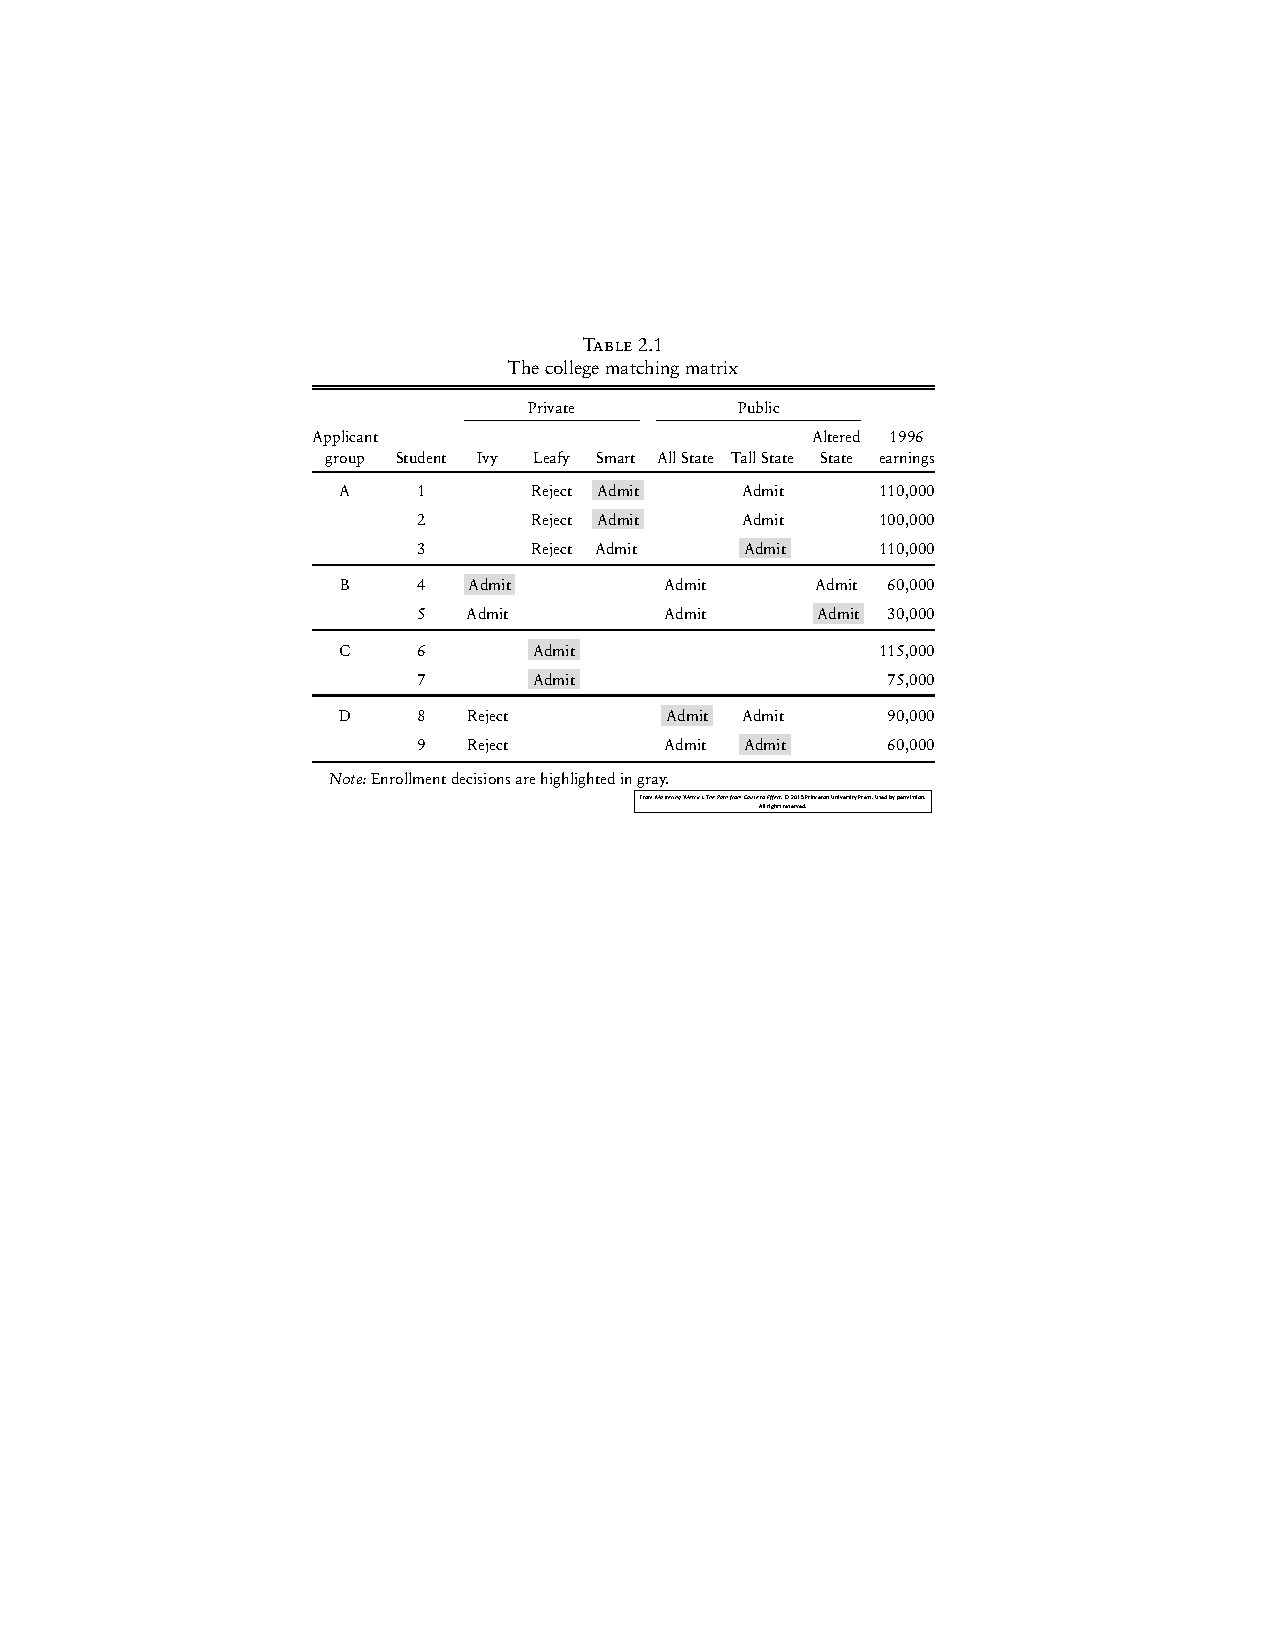
\includegraphics[ scale = 0.8]{figures/MMtbl21}
%	\end{figure}
%	\end{frame}
%	
%	\begin{frame}
%	\frametitle{Matching Strategy}
%	\begin{itemize}
%		\item Students 1,2,4,6,7 attended private schools
%			\begin{itemize}
%					\item Average income 92,000
%				\end{itemize}
%		\item Students 3,5,8,9 attended public schools
%			\begin{itemize}
%					\item Average income 72,500
%				\end{itemize}
%		\item Hence, it suggests that private schools have an advantage
%		\item But there is a selection bias: students are applying to different set of universities and got accepted in different set of university
%			\begin{itemize}
%					\item Other things are not equal
%				\end{itemize}
%		\item Let's have a closer look
%	\end{itemize}
%	\end{frame}
%	
%	\begin{frame}{Matching Strategy}
%	\begin{itemize}
%		\item Group $A$
%			\begin{itemize}
%					\item Everyone applied to Leafy, Smart and Tall State
%					\item Got rejected from Leafy, accepted at Smart and Tall State
%					\item Third student went to Tall State
%					\item Earnings differential: $\frac{(110,000 + 100,000)}{2} - 110,000 = -5,000$
%					\item Private school effect is negative
%				\end{itemize}
%		\item Group $B$
%			\begin{itemize}
%					\item Applied to Ivy, All State and Altered State
%					\item Admitted everywhere
%					\item Fourth student studies at Ivy and fifth studies at Altered
%					\item Private university effect: 60,000 - 30,000 =  30,000
%				\end{itemize}
%		\item Group $C$ and $D$ reveals nothing. Why?
%		\item Group $A$ and $B$ provide all action
%			\begin{itemize}
%					\item They include private and public university students
%					\item students were admitted to same set of schools
%				\end{itemize}
%	\end{itemize}
%	\end{frame}
%	
%	\begin{frame}
%	\frametitle{Matching Strategy}
%	\begin{itemize}
%		\item Causal effect of private university on earnings
%			$$\frac{30,000 - 5,000}{2} = 12,500 $$
%		\item We can do better by taking weighted average
%			$$\frac{3}{5} \times (-5,000) + \frac{2}{5} \times 30,000 = 9,000 $$
%		\item Think again, why this strategy is removing selection bias
%			\begin{itemize}
%					\item Within group students applied to same college and admitted to same college
%					\item Hence, their $Y_0$'s are (on average) the same
%				\end{itemize}
%		\item Rejecting the selection bias, and comparing private to public college earning will give us 19,500
%	\end{itemize}
%	\end{frame}
%	
%	\begin{frame}
%	\frametitle{Regression as a Matchmaker}
%	\small
%	\begin{itemize}
%		\item What did we learn till now from our very stylized example?
%			\begin{itemize}
%					\item Group $C$ and $D$ don't provide any information due to lack of variation
%					\item Group $A$ average income is higher than Group $B$
%				\end{itemize}
%		\item We can run the following regression
%			$$ Y_i = \alpha + \beta P_i  + \gamma A_i + \varepsilon_i$$
%		 	\begin{itemize}
%			 		\item $P_i$: dummy variable indicating attending private college
%			 		\item $A_i$: dummy variable indicating membership of group $A$
%			 		\item $\beta$ gives us the causal effect of treatment (attending private college)
%			 			\begin{itemize}
%				 				\item Note that our terming of $\beta$ as the causal effect of treatment is a conceptual issue based on research  question and empirical strategy
%				 			\end{itemize}
%			 	\end{itemize}
%	 	\item We can run regression for these 5 students and get
%	 		$$\alpha = 40,000\;\;\; \beta = 10,000 \;\;\; \gamma = 60,000 $$
%	 	\item $\beta$ value is close to what we got earlier but not close
%	 		\begin{itemize}
%		 			\item Regression assigns weights differently (discussed later)
%		 		\end{itemize}
%	\end{itemize}
%	\end{frame}
%	
%	\begin{frame}
%	\frametitle{Regression as a Matchmaker}
%	\begin{itemize}
%		\item So, regression, on a very basic level acts as this matchmaker
%		\item Just by including appropriate controls we are able to achieve matching
%	\end{itemize}
%	\end{frame}
%	
%	\begin{frame}
%	\frametitle{Digging Deeper: Coming Back to C\&B Data}
%	\begin{itemize}
%		\item 14,000 former students
%		\item Students were admitted and rejected at many different combination of schools
%		\item Many possible sets are represented by only one student
%		\item Some sets have more than one student, but all schools are either private or public (remember Group $C$ and $D$)
%		\item So this makes our life difficult
%	\end{itemize}
%	\end{frame}
%	
%	\begin{frame}
%	\frametitle{C\&B Data}
%	\begin{itemize}
%		\item Follow different strategy: group schools by their selectivity
%		\item Use Barron's selective categories
%		\begin{align*}
%			\text{Competitive} &\left\{ \begin{array}{c}
%				\text{All State} \\
%				\text{Tall State}
%				\end{array}\right.\\ 
%			\text{Highly Competitive} &\left\{ \begin{array}{c}
%				\text{Altered State} \\
%				\text{Smart State}
%				\end{array}\right.\\
%			\text{Most Competitive} &\left\{ \begin{array}{c}
%				\text{Leafy} \\
%				\text{Ivy}
%				\end{array}\right.
%			\end{align*}
%		\item New matching: 9,202 students
%		\item Focus on public-private universities: 5,583 students
%		\item Group into 151 similar selectivity groups1
%	\end{itemize}
%	\end{frame}
%	
%	\begin{frame}
%	\frametitle{New Regression}
%	$$\ln Y_i = \alpha + \beta P_i + \sum_{j=1}^{150}\gamma_j \text{GROUP}_{ji} + \delta_1 \text{SAT}_i + \delta \ln PI_i + \varepsilon_i $$
%	\begin{itemize}
%		\item Why use $\ln Y_i$ and not $Y_i$?
%	\end{itemize}
%	\end{frame}
%	
%	\begin{frame}
%	\frametitle{C\&B Data Results}
%	\begin{figure}
%		\centering
%		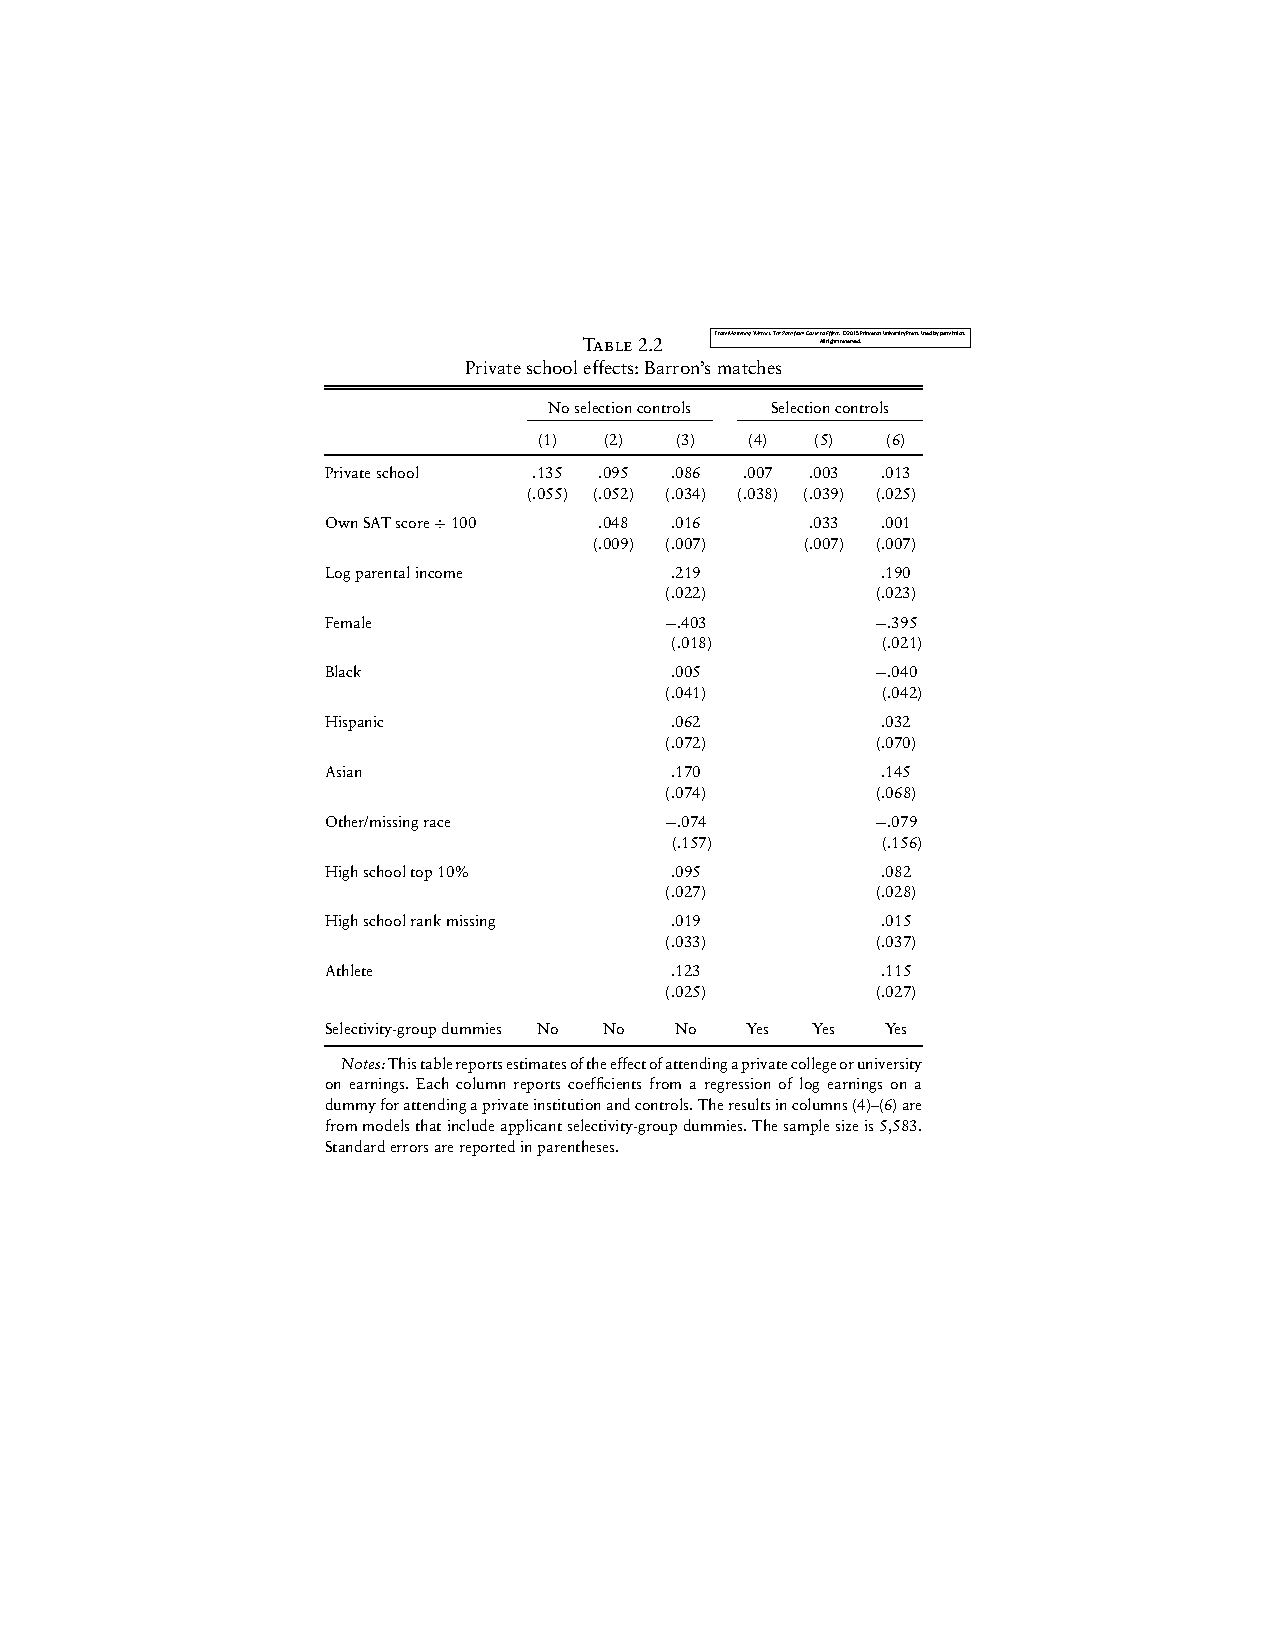
\includegraphics[ scale = 0.7]{figures/MMtbl22}
%	\end{figure}
%	\end{frame}
%	
%	\begin{frame}
%	\frametitle{C\&B Data Results}
%	\begin{figure}
%		\centering
%		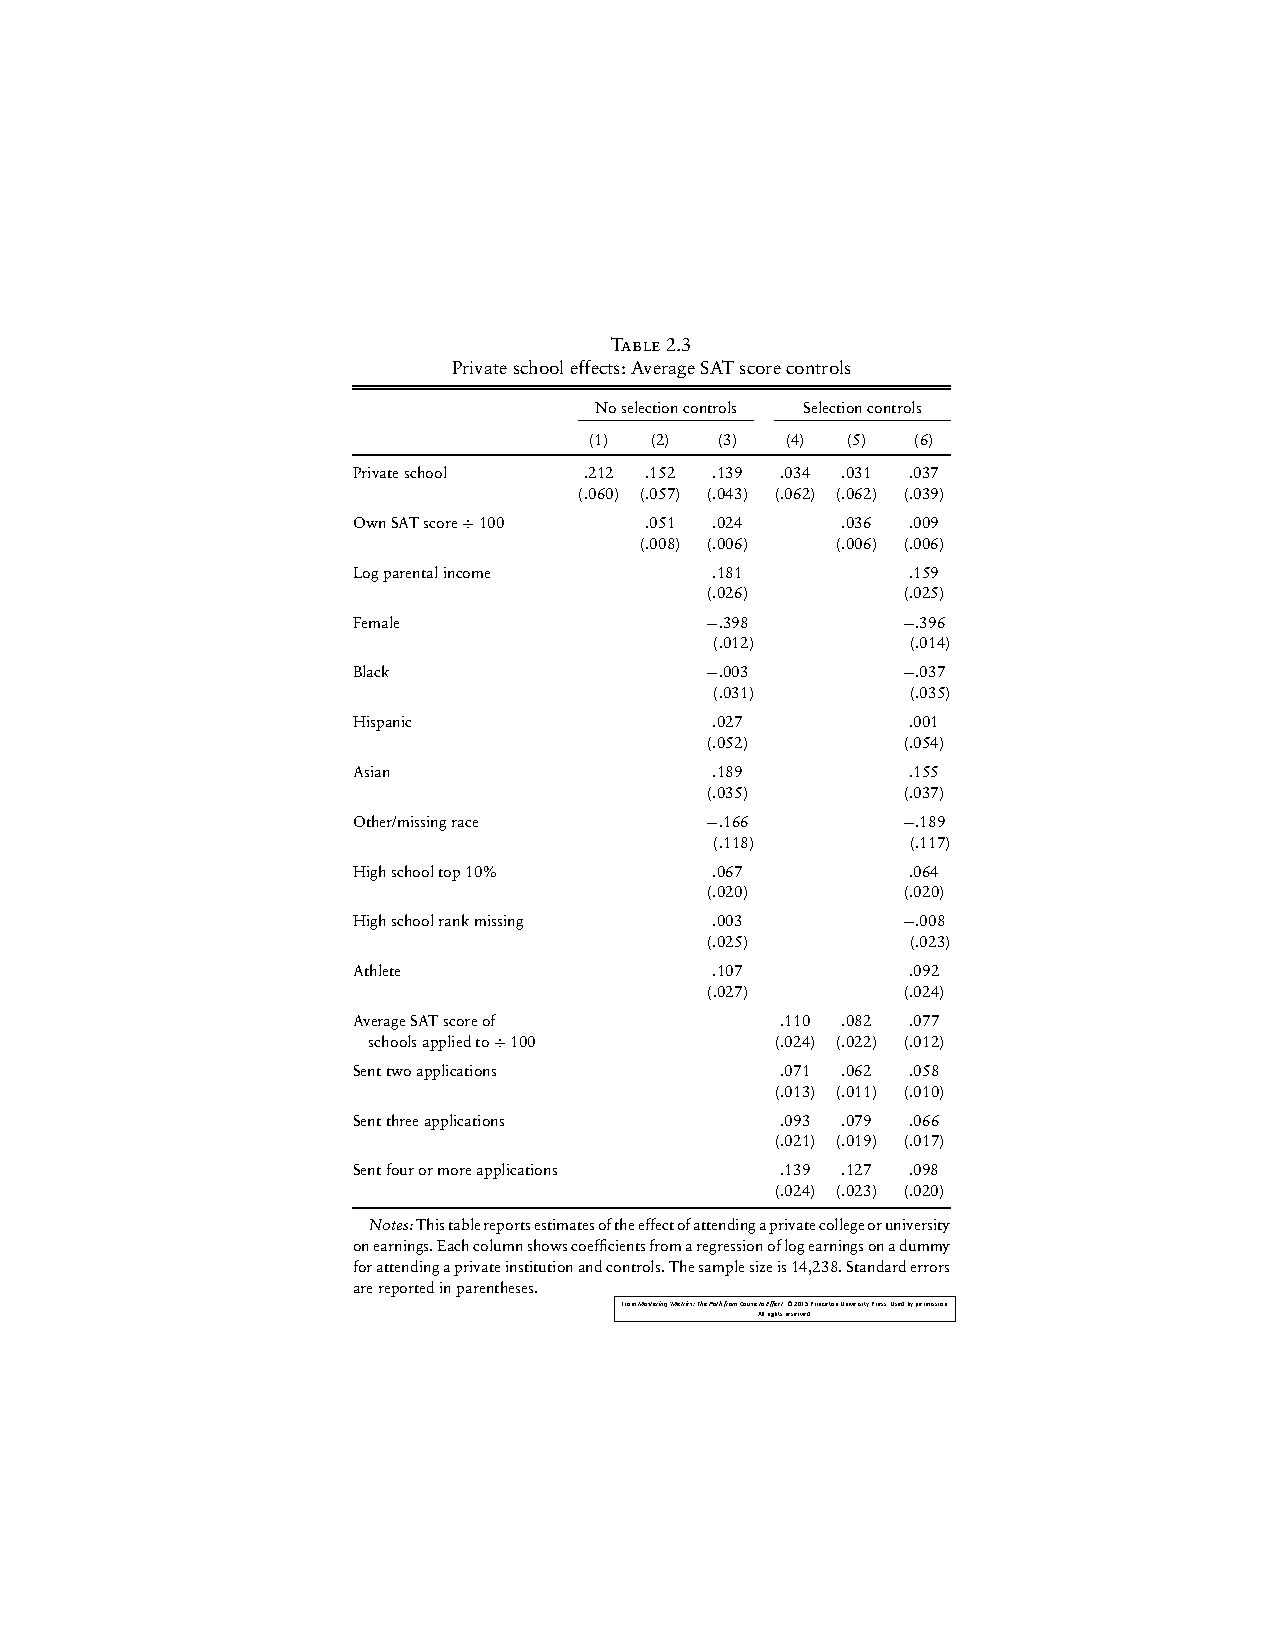
\includegraphics[ scale = 0.4]{figures/MMtbl23}
%	\end{figure}
%	\end{frame}
%	
%	
%	\begin{frame}
%	\frametitle{C\&B Data Results}
%	\begin{figure}
%		\centering
%		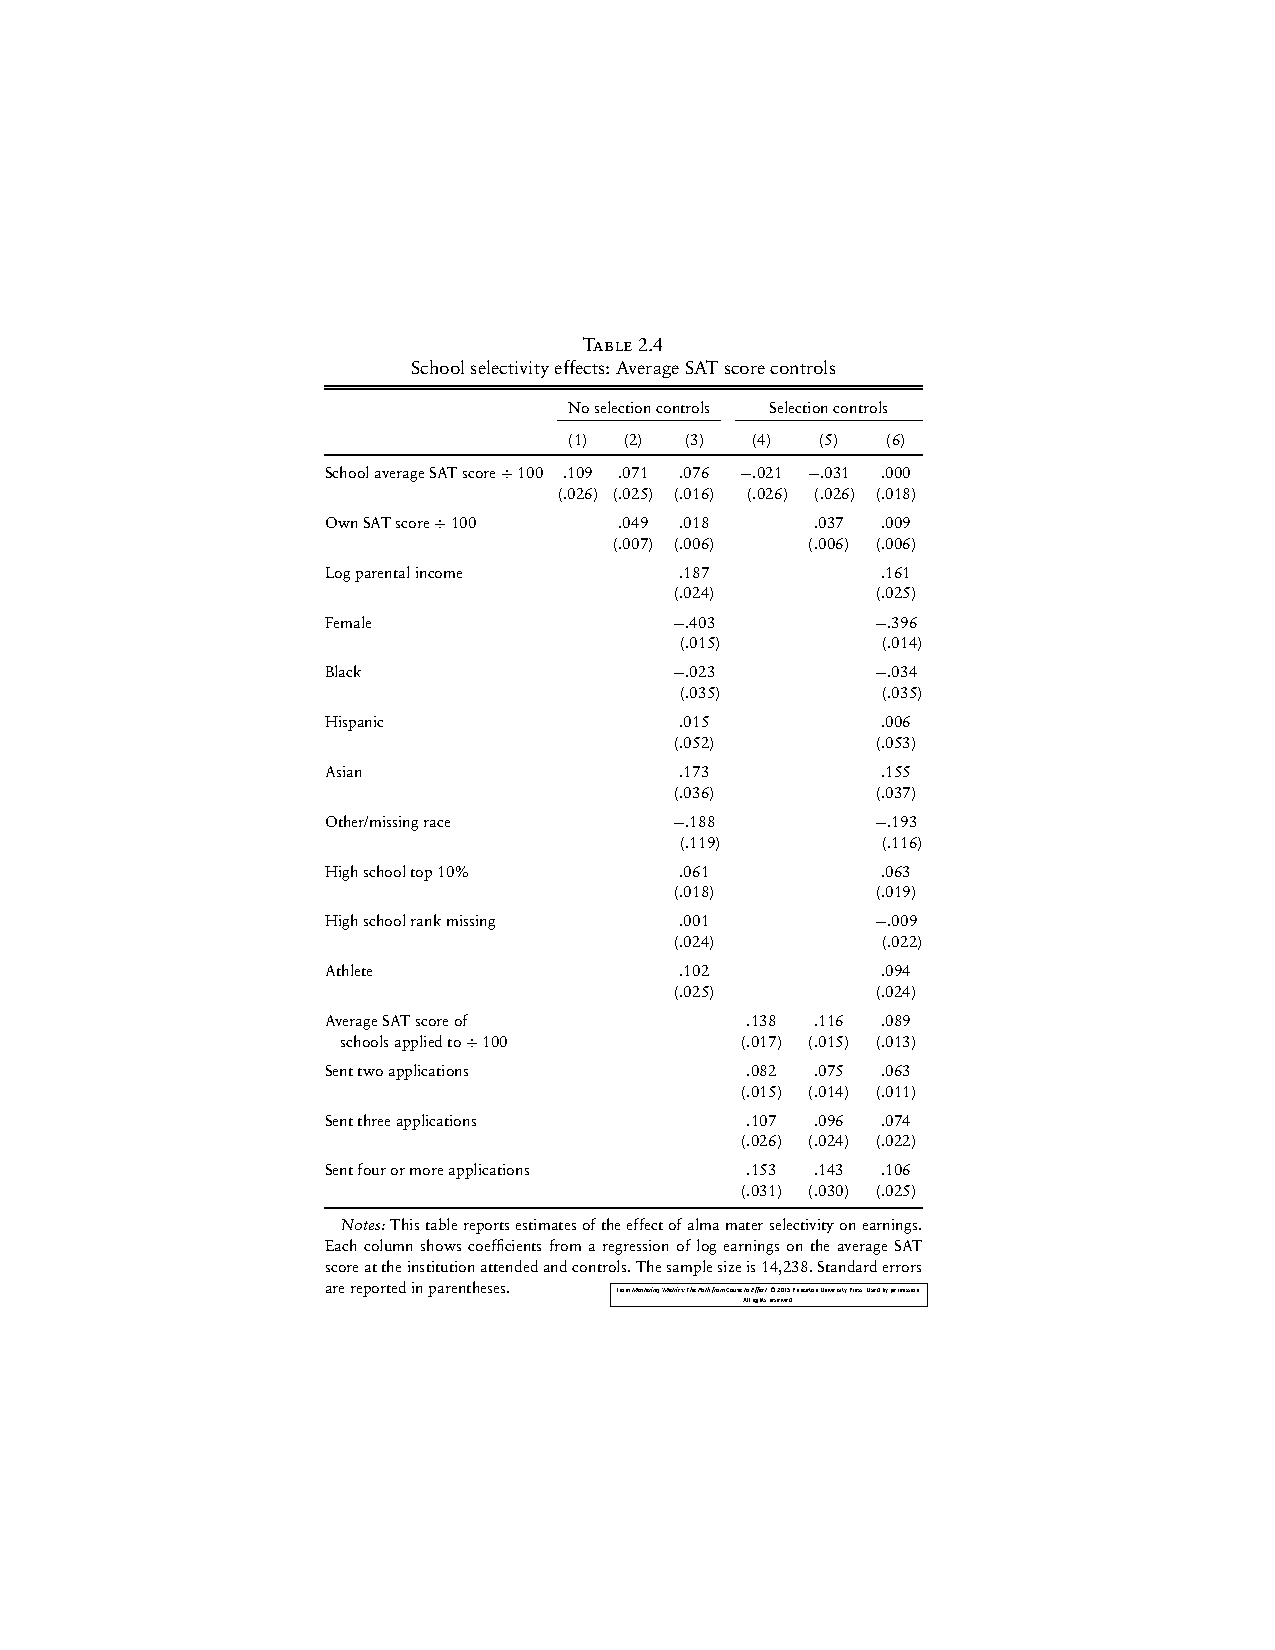
\includegraphics[ scale = 0.5]{figures/MMtbl24}
%	\end{figure}
%	\end{frame}
%	
%	\begin{frame}
%	\frametitle{Omitted Variable Bias (OVB)}
%	\begin{itemize}
%		\item Regression allows us to make other things equal
%		\item But only those things are equal for which we have control variables on the right hand side
%		\item Omission of control variables lead to OVB
%		\item Let's re-take the example of five students (Group $A$ and $B$)
%		\item Long regression 
%			$$ Y_i = \alpha^l + \beta^l P_i + \gamma A_i + e^L_i $$
%		\item Short regression ($A_i$ is omitted)
%			$$ Y_i = \alpha^s + \beta^s P_i + e^s_i $$
%		\item If you run this regression, you will get
%			$\beta^s = 20,000$ and $\beta^l = 10,000$
%		\item Hence $OVB = \beta^s - \beta^l = 20,000 - 10,000 = 10,000$
%	\end{itemize}
%	\end{frame}
%	
%	\begin{frame}
%	\frametitle{Omitted Variable Bias (OVB)}
%	\begin{figure}
%		\centering
%		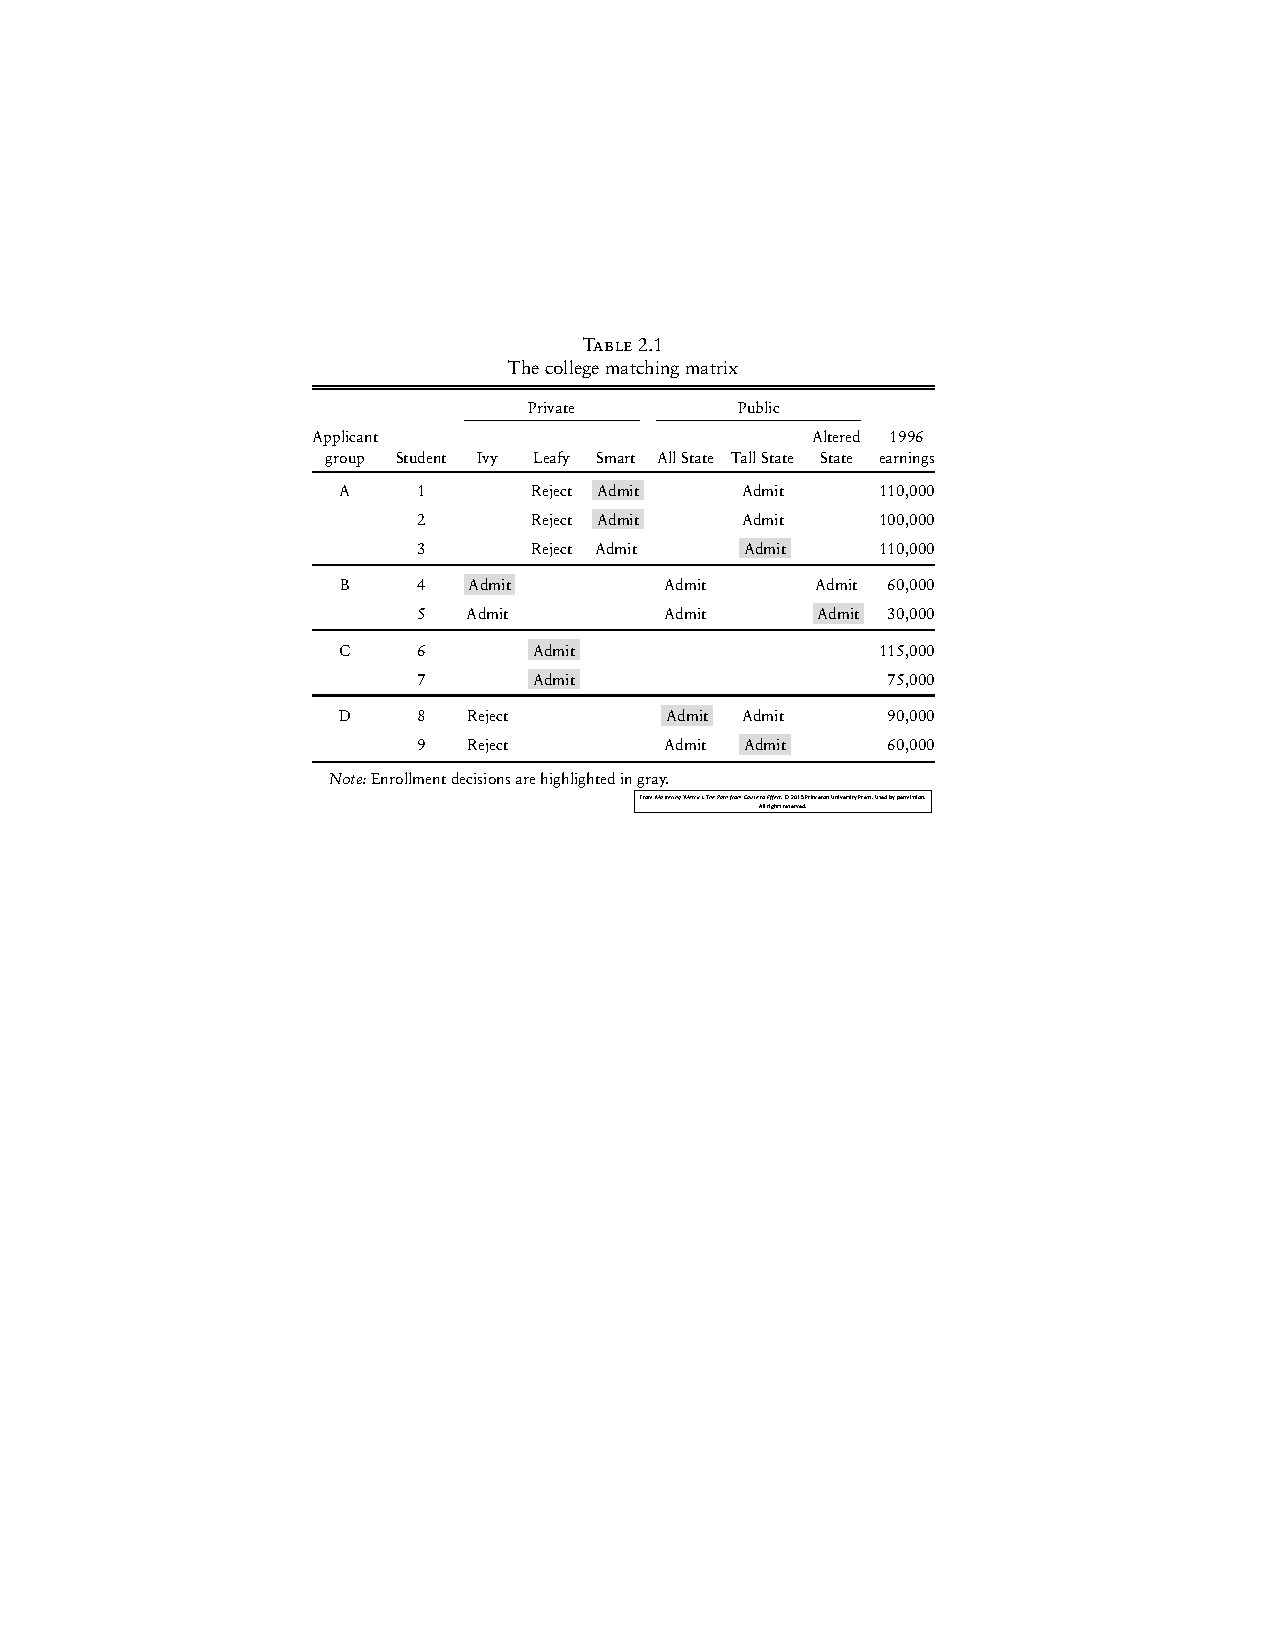
\includegraphics[ scale = 0.8]{figures/MMtbl21}
%	\end{figure}
%	\end{frame}
%	
%	
%	\begin{frame}
%	\frametitle{Omitted Variable Bias (OVB)}
%	\begin{itemize}
%		\item From where $OVB = 10,000$ is coming from?
%		\item Note two important observations
%			\begin{enumerate}
%					\item Average earnings of students in Group $A$ exceeds those from Group $B$
%					\item Two thirds of students in Group $A$ attend private school compared to fifty percent in Group $B$
%				\end{enumerate}
%		\item Dummy $A_i$ captures these two points
%	\end{itemize}
%	\end{frame}
%	
%	\begin{frame}
%	\frametitle{Omitted Variable Bias}
%	\tiny{
%	\begin{itemize}
%		\item Formally, relationship between $\beta^s$ and $\beta^l$ have two components
%
%			\begin{enumerate}
%					\item Relationship between $A_i$ (omitted variable) and treatment variable ($P_i$): two third students in Group $A$ attend private school
%					\item Relationship between $A_i$ (omitted variable) and outcome variable ($Y_i$): Group $A$ students on average earn more
%				\end{enumerate}
%		\item We get the following formula 
%
%			\begin{align*}
%				\text{Effect of } P_i \;\; \text{in short} &=  \text{Effect of } P_i \;\; \text{in long}+ \\ 
%				&(\{\text{Relationship between omitted and included}\} \times \\
%				& \{\text{Effect of omitted in long}\} )\\
%				&=  \text{Effect of } P_i \;\; \text{in long}+ \\ 
%				&(\{\text{Relationship between} \;\;P_i\;\; \text{and} A_i\} \times \\
%				& \{\text{Effect of}\;\; A_i\;\; \text{in long}\} )
%				\end{align*}
%		\item Hence OVB is given as
%			\begin{align*}
%				OVB  = (\{\text{Relationship between} \;\;P_i\;\; \text{and} A_i\} \times 
%				 \{\text{Effect of}\;\; A_i\;\; \text{in long}\} )
%				\end{align*}
%	\end{itemize}}
%	\end{frame}
%	
%	\begin{frame}
%	\frametitle{Omitted Variable Bias: Family Size ($FS$)}
%	\small
%	\begin{itemize}
%		\item Suppose family size is an omitted variable
%		\item Then 
%		$$ OVB  = (\{\text{Relationship between} \;\;P_i\;\; \text{and} FS_i\} \times 
%		\{\text{Effect of}\;\; FS_i\;\; \text{in long}\} )$$
%		\item Why family size is important?
%			\begin{itemize}
%					\item Smaller families are associated with higher earnings 
%					\item Private college students generally come from smaller families 
%				\end{itemize}
%		\item Two regressions
%			$$\ln Y_i = \alpha + \beta^l P_i + \sum_{j=1}^{150}\gamma^l_j \text{GROUP}_{ji} + \delta^l_1 \text{SAT}_i + \delta_2^l \ln PI_i + \lambda\; FS_i + \varepsilon_i  $$
%			$$FS_i = \pi_0 + \pi_1 P_i + \sum_{i=1}^{150}\theta_j \text{GROUP}_{ji} + \pi_2 \text{SAT}_i + \pi_3 \; \ln PI_i + u_i $$
%	\end{itemize}
%	\end{frame}
%	
%	\begin{frame}
%	\frametitle{Omitted Variable Bias: Family Size ($FS$)}
%	\begin{itemize}
%		\item $OVB = \beta - \beta^l = \pi_1 \times \lambda$
%		\begin{itemize}
%				\item $\pi_1 < 0$: students in private colleges are likely to come from smaller families
%				\item $\lambda < 0$: students from smaller families are likely to earn more
%			\end{itemize}
%		\item Hence $\beta - \beta^l > 0$
%		\item Note that in results, without including family size, causal effect of private college is small and insignificant
%		\item OVB formula tells us that these estimated causal effect are still too large because we are not including family size
%	\end{itemize}
%	\end{frame}

\begin{frame}
	\begin{center}
		\Large\textcolor{blue}{Regression: Mathematical Details}
	\end{center}
\end{frame}

	

\begin{frame}
	\frametitle{Population Model}
	\begin{itemize}
		\item Random sample of $(y,x)$ from the population
		\item \textbf{Objective:} Understand how $y$ changes with $x$?
		\item Linear model: $y = \beta_0 + \beta_1 x + u$
		\item Note that this model specification is an assumption
		\item What we mean by writing this type of specification?
		\begin{itemize}
			\item $x$ is affecting $y$ linearly, \textbf{but} 
			\item A host of other factors, captured by $u$ are also affecting
		\end{itemize}
	\end{itemize}
\end{frame}	


\begin{frame}
	\frametitle{Population Model: Assumption 1}
	\begin{assumption}\label{assu:ols-1}
		In population, $\mathbb E(u) = 0$.
	\end{assumption}
	
	\begin{itemize}
		\item This is an innocuous assumption
		\begin{align*}
			y &= \beta_0 + \beta_1 x + u \\
			&\equiv \beta_0 + \alpha_0 + \beta_1 x + u -\alpha_0 
		\end{align*}
		\item Note that changing intercept has no effect on $\beta_1$
	\end{itemize}
\end{frame}	


\begin{frame}
	\frametitle{Population Model: Assumption 2}
	\begin{assumption}
		$\mathbb E(u | x) = \mathbb E(u)$ for all values of $x$
	\end{assumption}
	\begin{itemize}
		\item Crucial assumption
		\item Not verifiable. Why?
	\end{itemize}
	
	\begin{example}
		Let's say $y$  is wage, and $x$ is years of schooling. What we don't observe is the ability of a person, which is subsumed in $u$. Essentially, with Assumption 2 we are saying:
		
		$$\mathbb E(u |x =1) = \mathbb E(u | x=16) $$
	\end{example}
	\pause
	\begin{itemize}
		\item If both assumptions hold,
		$$\mathbb E(u|x) = \mathbb E(u) = 0 $$
		\item Conditional expectation function \textcolor{red}{[Very important concept. Coming back to it later.]}
		$$\mathbb E(y|x) = \beta_0 + \beta_1x  $$
	\end{itemize}
\end{frame}



\begin{frame}
	\frametitle{Ordinary Least Squares (OLS)}
	\begin{itemize}
		\item \textbf{Question:} We have data on $x$ and $y$. How can we estimate $\beta_0$ and $\beta_1$?
		\item We have the following model
		\begin{align*}
			y_i &= \beta_0 + \beta_1 x_i + u_i, \;\;\; i=\{1,\cdots,n\}\\
			\mathbb E(u) &=0\\
			\mathbb E(u|x) &=0
		\end{align*}
		\item We \textbf{observe} $y$'s and $x$'s, but $u$ is never going to be observed
	\end{itemize}
	\begin{lemma}
		$\mathbb E(u\mid x) = 0$ implies $\mathbb E(ux) = 0$
	\end{lemma}
	\begin{proof}
		\begin{align*}
			\mathbb E(ux) &= \mathbb E[\mathbb E(ux\mid x)]\\
			&= \mathbb E[x\mathbb E(u\mid x)]\\
			&= 0
		\end{align*}
	\end{proof}
\end{frame}


\begin{frame}
	\frametitle{Ordinary Least Squares (OLS)}
	\begin{itemize}
		\item We have two unknowns -- $\beta_0$, $\beta_1$ -- and two equations
		\begin{align*}
			\mathbb E(u) &=0\\
			\mathbb E(ux) &=0
		\end{align*}
		\item We can further write
		\begin{align*}
			\mathbb E(y - \beta_0 -\beta_1 x) =0\\
			\mathbb E(x[y - \beta_0 -\beta_1 x]) =0
		\end{align*}
		\item Let's say we have $n$ observations, indexed by $i$, $(y_i,x_i)$
		\item Sample counterpart of two conditions is
		\begin{align*}
			&\frac{1}{n}\sum_{i=1}^n\left(y_i - \widehat\beta_0 - \widehat \beta_1 x_i \right)=0\\
			&\frac{1}{n}\sum_{i=1}^n\left(x_i\left[y_i - \widehat\beta_0 - \widehat \beta_1 x_i\right] \right)=0
		\end{align*}
		\item Notice the switch from $\beta_0, \beta_1$ to $\widehat \beta_0, \widehat \beta_1$
	\end{itemize}
\end{frame}

\begin{frame}
	\frametitle{Ordinary Least Squares}
	\begin{itemize}
		\item Solution of two equations will give
		\begin{align*}
			\widehat{\beta_0} &= \overline y - \widehat{\beta_1} \overline x\\
			\widehat{\beta_1} &= \frac{\sum_{i=1}^n (x_i - \overline x) (y_i - \overline y)}{\sum_{i=1}^n(x_i -\overline{x})^2} 
		\end{align*}
		\item You cannot identify $\widetilde{\beta_1}$ if $\sum_{i=1}^n(x_i -\overline{x})^2 = 0$
			\begin{itemize}
				\item When will this be the case?
			\end{itemize}
	\end{itemize}
\end{frame}




\begin{frame}
	\frametitle{Conditional Expectation Function (CEF)}
	\begin{itemize}
		\item CEF is given as $\mathbb E[Y_i | X_i]$ where $X_i$ is a $K \times 1$ vector of covariates
		\item Interpretation: population average of $Y_i$ keeping $X_i$ fixed
		\item Population average: mean in an infinitely large sample
		\item Note that expectation is a population concept.
		\begin{itemize}
			\item What is the difference between population and sample?
		\end{itemize}
	\end{itemize}
\end{frame}

\begin{frame}
	\frametitle{Conditional Expectation Function (CEF)}
	\begin{figure}
		\centering
		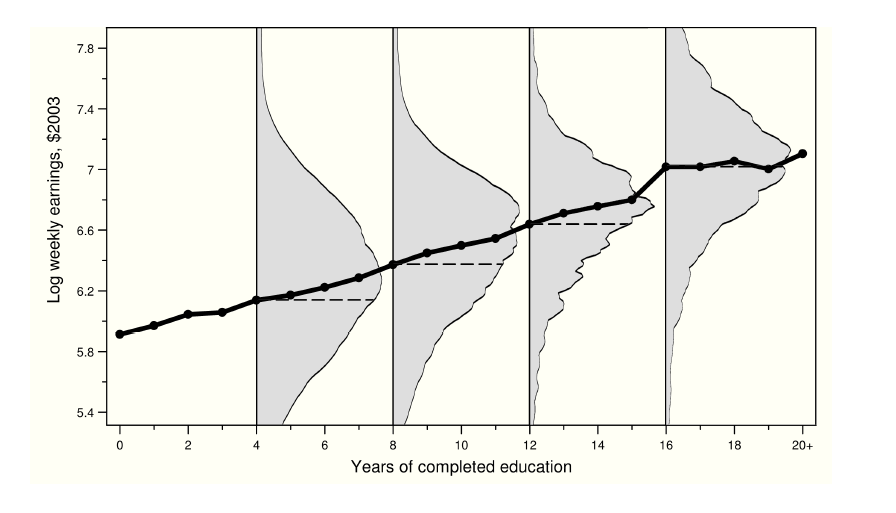
\includegraphics[width=\linewidth]{figures/mhe_fig_311}
	\end{figure}
\end{frame}

\begin{frame}{Conditional Expectation Function (CEF)}
	\begin{itemize}
		\item CEF at $X_i = x$ is given as
		$$\mathbb E[Y_i | X_i = x] = \int t f_y(t | X_i = x) dt $$
		\item Using the law of iterated expectations, the unconditional average of $Y_i$ can be derived as the unconditional average of CEF
		$$\mathbb E[Y_i] = \mathbb E\left\{ \mathbb E[Y_i | X_i]  \right\} $$
		where the outer expectation is on the distribution of $X_i$
		\begin{proof}
			Assume $(X_i, Y_i)$ are continuously distributed with $f_{xy}(u,t)$ where $f_y(t | X_i = u)$ is the conditional distribution of $Y_i$ given $X_i = u$ and $g_y(t)$ and $g_x(u)$ are marginal densities
		\end{proof}
	\end{itemize}
\end{frame}


\begin{frame}{Conditional Expectation Function (CEF)}
	\begin{align*}
		\mathbb E \left\{ \mathbb E[Y_i| X_i]  \right\} &= \int \mathbb E[Y_i | X_i = u] g_x(u) \operatorname{d}u\\
		&= \int \left[ \int t f_y(t|X_i = u) \operatorname{d}t \right] g_x(u) \operatorname{d}u\\
		&= \int\int t f_y(t | X_i = u) g_x(u) \operatorname{d}u\\
		&= \int t \left[\int f_y(t | X_i = u) g_x(u)\operatorname{d}u \right]\operatorname{d}t\\
		&= \int t \left[f_{xy}(u,t)\operatorname{d}u \right]\operatorname{d}t\\
		&= \int t g_y(t) \operatorname{d}t \\
		&= \mathbb E[Y_i]
	\end{align*}
\end{frame}


\begin{frame}
	\frametitle{Three Theorems of CEF}
%	\begin{theorem}[1. The CEF Decomposition Property ]
%		$$ Y_i = \mathbb E[Y_i | X_i] + \varepsilon_i$$
%		where (i) $\varepsilon_i$ is mean dependent of $X_i$ i.e. $\mathbb E[\varepsilon_i| X_i] = 0, and (ii) \varepsilon_i$ is uncorrelated with any function of $X_i$
%	\end{theorem}
\customtheorem{1. The CEF Decomposition Property}{$$ Y_i = \mathbb E[Y_i | X_i] + \varepsilon_i$$
	where (i) $\varepsilon_i$ is mean dependent of $X_i$ i.e. $\mathbb E[\varepsilon_i| X_i] = 0, and (ii) \varepsilon_i$ is uncorrelated with any function of $X_i$}
	\begin{proof}
		For the first point:
		\begin{align*} 
			\mathbb E[\varepsilon_i | X_i] &= \mathbb E[Y_i - \mathbb E[Y_i|X_i] | X_i]\\
			&= \mathbb E[Y_i | X_i] - \mathbb E[Y_i | X_i] = 0
		\end{align*}
		For the second point let $h(X_i)$ be any function of $X_i$. Then
		\begin{align*}
			\mathbb E[h(X_i)\varepsilon_i] &= \mathbb E\left\{\mathbb E[h(X_i)\varepsilon_i|X_i]\right\}\\
			&= \mathbb E\left\{ \mathbb{E} [h(X_i)] \mathbb E(\varepsilon_i|X_i) \right\}\\
			&= 0
		\end{align*}
		where first equality uses law of iterated expectations.
	\end{proof}
\end{frame}

\begin{frame}
	\frametitle{Three Theorems of CEF}
	\begin{itemize}
		\item Intuitively, Theorem 1 says  that any random variable $Y_i$ can be decomposed into two parts
		\begin{enumerate}
			\item one which is explained by $X_i$ i.e. $\mathbb E[Y_i|X_i]$
			\item and the left over piece which is orthogonal to $X_i$ by construction
		\end{enumerate}
	\end{itemize}
\end{frame}

\begin{frame}
	\frametitle{Three Theorems of CEF}
%	\begin{theorem}[2. The CEF Prediction Property]
%		Let $m(X_i)$ be any function of $X_i$. The CEF solves 	
%		$$ \mathbb E[Y_i| X_i] = \arg min_{m(X_i)} \mathbb E[(Y_i - m(X_i))^2] $$
%		Hence CEF is the minimum mean square estimator of $Y_i$ given $X_i$
%	\end{theorem}

\customtheorem{2. The CEF Prediction Property}{		Let $m(X_i)$ be any function of $X_i$. The CEF solves 	
	$$ \mathbb E[Y_i| X_i] = \arg min_{m(X_i)} \mathbb E[(Y_i - m(X_i))^2] $$
	Hence CEF is the minimum mean square estimator of $Y_i$ given $X_i$
}
	
	\begin{proof}
		\begin{align*}
			[Y_i - m(X_i)]^2 &= \left( [Y_i - \mathbb E(Y_i|X_i)] + [\mathbb E(Y_i|X_i) - m(X_i)] \right)^2\\
			&= (Y_i - \mathbb E[Y_i | X_i])^2 + 2(\mathbb E[Y_i|X_i] - m(X_i))(Y_i - \mathbb E[Y_i|X_i])  + \\ &\qquad\qquad\qquad\qquad (\mathbb E[Y_i|X_i] - m(X_i))^2
		\end{align*}
		The second term can be written as $h(X_i)\varepsilon_i$ where $h(X_i) = 2(\mathbb E[Y_i|X_i] - m(X_i))$ which will have expectation zero by Theorem 1. The last term is zero when $m(X_i) = \mathbb E[Y_i|X_i]$
	\end{proof}
	
	%\begin{theorem}[3. ANOVA Theorem]
	%	$$\operatorname{var}[Y_i] = \operatorname{var}[\mathbb E(Y_i|X_i)] + \mathbb E [\operatorname{var}(Y_i | X_i)] $$
	%\end{theorem}
\end{frame}


\begin{frame}
	\frametitle{Three Theorems of CEF}
%	
%	\begin{theorem}[3. ANOVA Theorem]
%		$$\operatorname{var}[Y_i] = \operatorname{var}[\mathbb E(Y_i|X_i)] + \mathbb E [\operatorname{var}(Y_i | X_i)] $$
%	\end{theorem}

\customtheorem{3. ANOVA Theorem}{$$\operatorname{var}[Y_i] = \operatorname{var}[\mathbb E(Y_i|X_i)] + \mathbb E [\operatorname{var}(Y_i | X_i)] $$}
	
	\begin{proof}
		By theorem 1:
		\begin{align*}
			Y_i &= \mathbb E[Y_i | X_i]+ \varepsilon_i\\
			\operatorname{var}(Y_i) &= \operatorname{var} (\mathbb E[y_i|X_i]) + \operatorname{var}(\varepsilon_i)\\
		\end{align*}
		Now $\operatorname{var}(\varepsilon_i)$ can be written as
		\begin{align*}
			\operatorname{var}(\varepsilon_i) &= \mathbb E[\varepsilon_i^2]\\
			&= \mathbb E[\mathbb E(\varepsilon_i^2|X_i)]\\
			&= \mathbb E[\mathbb{E}([Y_i - \mathbb E(Y_i|X_i)]^2|X_i)]\\
			&= \mathbb E[ \mathbb E(Y_i^2 | X_i) - \mathbb E(Y_i|X_i)^2]\\
			&= \mathbb E[\operatorname{var}(Y_i|X_i)]
		\end{align*}
	\end{proof}
\end{frame}


\begin{frame}
	\frametitle{Regression and CEF}
	\begin{itemize}
		\item Regression function: the best fitting line generated by minimizing expected square errors
		\item So what is the relationship between the regression function (which has a restricted functional form) and the CEF (which does not)
	\end{itemize}
\end{frame}


\begin{frame}
	\frametitle{Regression Anatomy}
	\begin{itemize}
		\item Let $\beta$ be a $K \times 1$ vector of regression coefficients obtained by solving
		\begin{align}\label{regeq}
			\beta = \argmin_b  \;\;\;\mathbb E[(Y_i - X_i'b)^2]
		\end{align}
		\item The first order condition for this problem is 
		$$\mathbb E[X_i(Y_i - X_i'b)] = 0 $$
		which gives $\beta = \mathbb E[X_iX_i']^{-1}\mathbb E[X_iY_i]$
		\item In a simple bivariate case i.e. $K = 1$,  slope coefficient is $\beta_1 = \frac{\operatorname{cov}(Y_, X_i)}{\operatorname{var}(X_i)}$ and constant is given as $\alpha = \mathbb E[Y_i] - \beta_1 \mathbb E[X_i]$
		\item For $K > 1$, the $k^{th}$ coefficient is given as 
		\begin{align}\label{reganatomy}
			\beta_k =\frac{\operatorname{var}(Y_i, \widetilde{x}_{ki})}{\operatorname{var}(\widetilde{x}_{ki})}
		\end{align}
		where $\widetilde{x}_{ki}$ is the residual from a regression of $x_{ki}$ on all other covariates 
	\end{itemize}
\end{frame}

\begin{frame}
	\frametitle{Regression Anatomy}
	\begin{itemize}
		\item Regression anatomy formula \eqref{reganatomy} is more intuitive than matrix notation \eqref{regeq}
		\begin{itemize}
			\item Each coefficient in a multivariate regression is the bivariate slope coefficient for the corresponding regressor after partialling out all other covariates
		\end{itemize}
		\item Now we move onto the point which Mostly Harmless Econometrics captures very nicely 
		\begin{quote}
			you should be interested in the regression parameters if you are interested in the CEF
		\end{quote}
	\end{itemize}
\end{frame}

\begin{frame}
	\frametitle{Three theorems (without proofs)}
	\customtheorem{1. The Linear CEF Theorem [Regression Justification 1]}{
		Suppose the CEF is linear. Then the population regression function is it.}
	\begin{itemize}
		\item This means if the CEF is linear then it will be captured by the regression function.
		\item Question is: when CEF is linear?
		\begin{enumerate}
			\item When vector $(Y_i, X_i')$ has a multivariate normal distribution
			\item When regression is saturated:
			\begin{itemize}
				\item a saturated regression model has a separated parameter for every possible combination of values that the set of regressors take on
			\end{itemize}
		\end{enumerate}
	\end{itemize}
\end{frame}

\begin{frame}
	\frametitle{Three Theorems (without proofs)}
	\customtheorem{2. The Best Linear Predictor Theorem [Regression Justification 2]}{
	\\	The function $X_i'\beta$ is the best linear predictor of $Y_i$ given $X_i$ in a MMSE sense.}
	\begin{itemize}
		\item Among \textbf{all} functions, CEF $E[Y_i|X_i]$ is the best predictor of $Y_i$ given $X_i$
		\item Among \textbf{linear} functions, the regression function $X_i'\beta$ is the best predictor of $Y_i$ given $X_i$
	\end{itemize}
\end{frame}

\begin{frame}
	\frametitle{Three Theorems (without proofs)}
\customtheorem{3. The Regression CEF Theorem [Regression Justification 3]}{
		\\The regression function provides minimum mean square error (MMSE) approximation to $\mathbb E[Y_i|X_i]$, that is,
		$$ \beta = \argmin_b \mathbb E[(E[Y_i|X_i] - X_i'b)^2]$$}

	\begin{itemize}
		\item This theorem says that even if actual CEF is non-linear, regression provides the best linear approximation to it
	\end{itemize}
\end{frame}

\begin{frame}
	\frametitle{CEF and Regression}
	\begin{figure}
		\centering
		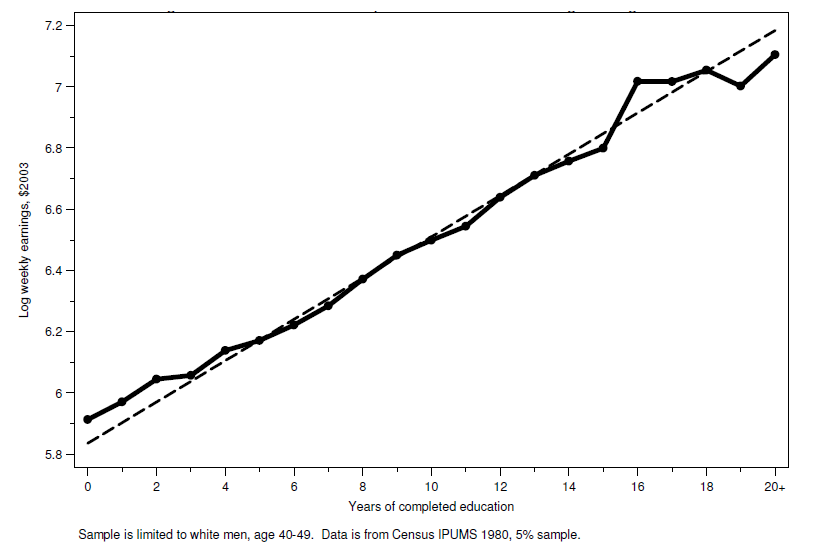
\includegraphics[width=\linewidth]{figures/mhe_fig_312}
	\end{figure}
\end{frame}

\begin{frame}
\frametitle{Regression and Causality}
\begin{itemize}
	\item From previous discussion: regression gives the best MMSE linear approximation to the CEF
	\item However, we still don't know when regression has a causal interpretation
	\item Let's go to the example of earnings and education
	\item Assume that the schooling is a binary decision:
		\begin{itemize}
				\item Going to the college, $C_i = 1$
				\item Not going to the college, $C_i = 0$
			\end{itemize}
	\item Potential outcome
		\begin{align*}
			= \left\{\begin{array}{cc}
				Y_{1i} & \text{if} \;\; C_i = 1\\
				Y_{0i} & \text{if} \;\; C_i = 0\\
				\end{array} \right.
			\end{align*}
\end{itemize}
\end{frame}

\begin{frame}
\frametitle{Regression and Causality}
\begin{itemize}
	\item Blind comparison of earnings of college goers (not-goers) will lead to 
	\begin{align*}
			\mathbb E[Y_i | C_i = 1] - \mathbb E[Y_i | C_i = 0] &= \mathbb E[Y_{1i} | C_i = 1] - \mathbb E[Y_{0i} | C_i = 0]\\
			&= \underbrace{\mathbb E[Y_{1i} | C_i = 1] - \mathbb E[Y_{0i} | C_i = 1]}_{\text{ATET}} +\\
			& \underbrace{\mathbb E[Y_{0i} | C_i = 1] - \mathbb E[Y_{0i} | C_i = 0]}_{\text{selection bias}}
		\end{align*}
	\item Here selection bias is positive, why?
\end{itemize}
\end{frame}

\begin{frame}
\frametitle{Conditional Independence Assumption (CIA)}
\begin{itemize}
	\item How can we eliminate the selection bias?
	\item Invoke the conditional independence assumption (CIA)
	\item CIA asserts that conditional on observed characteristics $X_i$, selection bias disappears
		$$\{Y_{0i}, Y_{1i}\} \independent C_i \rvert X_i  $$
	\item Hence, 
	\small
		\begin{align*}
				\mathbb E[Y_i | X_i, C_i = 1] - \mathbb E[Y_i | X_i, C_i = 0] &= \mathbb E[Y_{1i} | X_i, C_i = 1] - \mathbb E[Y_{0i} | X_i, C_i = 0]\\
				&= \mathbb E[Y_{1i} - Y_{0i} | X_i]
			\end{align*}
\end{itemize}
\end{frame}


\begin{frame}
\frametitle{Causal Interpretation under continuous variable}
\begin{itemize}
	\item Denote $Y_{si} = f_i(s)$ as the \textbf{potential} earnings that person $i$ would receive for $s$ years of education
	\item The CIA will become 
	$$ Y_{si} \independent s_i \rvert X_i $$
	\item Hence 
	\begin{align*}
		&\Rightarrow \mathbb E[Y_{i} | X_i, s_i = s] - \mathbb E[Y_{i} | X_i, s_i = s-1]\\
		 &\Rightarrow \mathbb E[Y_{si} | X_i, s_i = s] - \mathbb E[Y_{(s-1)i} | X_i, s_i = s-1]\\
		 &\Rightarrow \mathbb E[f_i(s) - f_i(s-1) | X_i]
		\end{align*}
\end{itemize}
\end{frame}

\begin{frame}
\frametitle{Regression and CIA}
\begin{itemize}
	\item Regression provides a way to turn CIA into causal estimate
	\item For now, assume, $f_i(s)$ is both linear in $s$ and same for everyone except for an additive error term
	\item In this case, linear constant effects causal model is given as 
	$$ f_i(s) = \alpha + \rho s + \eta_i$$
	\item Two points to note:
		\begin{enumerate}
				\item functional relationship is same for everyone, except for $\eta_i$
				\item this equation is a causal model in the sense that it is relating $s$ to potential outcomes
			\end{enumerate}
	\item If we replace $s$ with observed value we will get 
		$$ Y_i = \alpha + \rho s_i + \eta_i $$
	\item Due to selection bias, $s_i$ and $\eta_i$ may be correlated
\end{itemize}
\end{frame}

\begin{frame}
\frametitle{Regression and CIA}
\begin{itemize}
	\item Suppose CIA holds given a vector of observed co-variates $X_i$
	\item Decompose the random part of potential earnings $\eta_i$ into a linear function of observable characteristics $X_i$ and an error term $\nu_i$
		$$\eta_i = X_i'\gamma + \nu_i $$
	such that $\mathbb E[\eta_i | X_i] = X_i'\gamma$
	\item Then
		\begin{align*}
			\mathbb E[f_i(s)| X_i, s_i] &= \mathbb E[f_i(s)| X_i]\\
										&= \alpha + \rho s + \mathbb E[\eta_i | X_i]\\
										&= \alpha + \rho s + X_i'\gamma
			\end{align*}
\end{itemize}
\end{frame}

\begin{frame}
\frametitle{Regression and CIA}
\begin{itemize}
	\item Hence, residual in the linear causal model,
	 	$$ Y_i = \alpha + \rho s + X_i'\gamma + \nu_i $$
	 is uncorrelated with $s_i$ and $X_i$ and $\rho$ is the causal effect of interest
	 \item Take a note of an important assumption: $X_i$ is the reason why $s_i$ and $\eta_i$ are uncorrelated
	 \item What if some observable characteristics are missing?
	 	\begin{itemize}
	 		\item If missing characteristic correlated with inlcuded $X_i$ $\Rightarrow$ omitted variable bias
	 	\end{itemize}
\end{itemize}
\end{frame}

%\begin{frame}
%	\frametitle{Regression and Causality}
%	\begin{itemize}
%		\item We know what is regression giving us:
%		\begin{itemize}
%			\item Best linear approximation to the CEF
%		\end{itemize}
%		\item What we don't know:
%		\begin{itemize}
%			\item When regression has a causal interpretation?
%		\end{itemize}
%		\item Convoluted answer: regression is causal when CEF it approximates is causal
%		\begin{itemize}
%			\item Not an informative answer
%			\item Let's dig deeper
%		\end{itemize}
%		\item When is CEF causal?
%		\begin{itemize}
%			\item When it describes differences in average potential outcome for a fixed reference population
%		\end{itemize}
%		\item We will come back to this point again
%	\end{itemize}
%\end{frame}
%
%\begin{frame}
%	\frametitle{Conditional Independence Assumption (CIA)}
%	\begin{itemize}
%		\item Also called ``selection-on-observables''
%		\item Retain the example of education and earnings
%		\item However, for now make life easier, and think of education as a binary variable 
%		\begin{itemize}
%			\item Either I go to college, or I don't
%			\item Denote the decision to go to college by $C_i$
%			\begin{align*}
%				C_i = \left\{\begin{array}{ll}
%					1 & \;\;\; i\;\; \text{attends college}\\
%					0 & \;\;\; i\;\; \text{does not attend college}\\
%				\end{array}\right.
%			\end{align*}
%			\item Potential outcomes
%			\begin{align*}
%				\left\{\begin{array}{ll}
%					Y_{1i} & \;\;\text{if}\; C_i=1\\
%					Y_{0i} & \;\;\text{if}\; C_i=0\\
%				\end{array}\right.
%			\end{align*}
%			\item Causal effect
%			$$\delta_i =  Y_{1i} - Y_{0i} $$
%			\item What we hope to measure:
%			\begin{align*}
%				ATE &= \mathbb E[\delta_i]\\
%				ATT &= \mathbb E[\delta_i| C_i = 1]
%			\end{align*}
%		\end{itemize}
%	\end{itemize}	
%\end{frame} 




\end{document}